
\clearpage
%%%%%%%%%%%%%%%%%%%
\section{Introduction}
The question of how genetic variation is maintained, despite the effects of selection and drift, continues to be central to the study of evolutionary biology \citep{walsh_evolution_2018}. Classical explanations include overdominance (heterozygote advantage) or frequency-dependent selection, but in the modern era of genomic data, all patterns of variation that exceed the expected variation under neutrality tend to be categorized broadly as balancing selection, regardless of the evolutionary mechanism \citep{mitchell-olds_which_2007}.  One of the evolutionary mechanisms coined under balancing selection is sexually antagonistic selection, which occurs when the direction of natural selection on traits or loci differs between the sexes \citep{lande1980sexual,arnqvist2013sexual}.

Sexually antagonistic selection can in some cases can mantain polymorphisms of otherwise dis-advantageous alleles in a population \citep{gavrilets2014sexual}, which in turn can result in phenotypically distinct sexes that express  morphological, physiological, and behavioral traits to different degrees \citep{mori2017sexual,connallon2018environmental}. However,  sexually antagonistic selection can only mantain polymorphism in specific scenarios, as classical predictions show that sexual antagonism often results in the fixation of the fitter allele \citep{kidwell1977regions,pamilo1979genic,hedrick1999antagonistic,curtsinger1994antagonistic, patten2010fitness} . Importantly, the effect of sexually antagonistic selection, has been generally studied under strong simplifying assumptions such as constant population sizes and homogeneous environments (e.g., \citet{kidwell1977regions, pamilo1979genic, immler2012ploidally}). Few studies have explored the effect of sexually antagonistic selection on the maintenance of polymorphism with more realistic assumptions. Excepctions include \citet{connallon_evolutionary_2018} who found that classical predictions break down when fluctuations in the environment combined with life-history traits allow local adaptations and promote the maintenance of genetic diversity. The effect of environmental fluctuations without local adaptation, however, has not been studied in the context of sexually antagonistic selection to the best of our knowledge.


The contribution of environmental fluctuations to genetic variability remains a debated issue in evolutionary biology. Classic theoretical models predict that temporal fluctuations in environmental conditions are unlikely to maintain a genetic polymorphism \citep{hedrick1974genetic,hedrick1986genetic}. However, other studies have found that fluctuating selection can maintain genetic variance on sex--linked traits \citep{reinhold2000maintenance}, or in populations where generations overlap \citep{ellner1994role, ellner1996patterns}. Similarly, temporal changes in population sizes have been shown to mitigate the effect of genetic drift in small populations \citep{pemberton1996maintenance}, and in annual plant systems \citep{nunney2002effective}. Thus, both fluctuations in selection and population sizes could dramatically change the effect of sexually antagonistic selection in the maintenance of genetic diversity.


Importantly, progress requires more than just identifying if environmental fluctuations can maintain genetic diversity in a population, but to quantify how exactly they contribute to its maintenance \citep{ellner2016quantify}. Modern coexistence theory provides a powerful conceptual framework to do so \citep{Chesson2000,chesson1994multispecies, barabas_chessons_2018}. Although its core ideas were formalized in an ecological context \citep{chesson1994multispecies,Chesson2000}, this framework provides the necessary tools to examine the relative contributions of fluctuations to diversity maintenance, which can also be applied to evolutionary contexts  \citep{ellner1996patterns,reinhold2000maintenance,schreiber2020factors}. From an ecological perspective, polymorphism of sexually antagonistic alleles is equivalent to the coexistence of species, and the fixation of either one of the alleles in a population is equivalent to competitive exclusion. The coexistence of alleles, thus, can be examined through the same lens as the coexistence of competing species.

Here, we seek to explicitly apply recent  advances in modern coexistence theory to the question of how
polymorphism is maintained under sexually antagonistic selection.  We examined how fluctuations in selection values, fluctuations in population sizes, and their interactions can stabilize or hinder the coexistence of alleles. In particular, we examined  i) Can fluctuations in population sizes and selection values allow sexually antagonistic alleles to coexist when differences in their fitness would typically not allow them to? and ii) What is the relative contribution of different types of fluctuations that allow two sexually antagonistic alleles to be maintained in a population? Our study provides the tools to analyze evolutionary dynamics from a novel perspective and contributes to answering long-lasting questions regarding the effect of non-constant environments on genetic diversity.



\section{Methods}

We first present  a model that describes the evolutionary dynamics of sexually antagonistic alleles and show how changes in allele frequencies can be expressed in terms of growth rates, a necessary condition for analyses done using modern coexistence theory. We continue by simulating different scenarios of alleles invading a population, where we allowed population sizes, selection, both, or neither to vary. Finally, we examine the results of our simulations through a modern coexistence theory lens by calculating the contribution of each of these fluctuations in the coexistence of alleles.


\subsection*{Population dynamics of sexually antagonistic alleles}

 Our model considered evolution at single, biallelic  locus with frequency and density independent effects on the relative fitness of females and males. We examined the dynammics of two  sexually antagonistic alleles, $j$ and $k$, that affect fitness in the haploid state. We assumed allele $j$ always has a high fitness in females ($w_{jf} = 1$), but variable fitness in males ($w_{jm} < 1$); and allele $k$ has a high fitness in males ($w_{km} = 1$), but variable fitness in females ($w_{kf} < 1 $). The selection against allele $j$ in males is therefore $S_{m}= 1 - w_{jm}$, and the selection against allele $k$ in females is $S_{f}= 1 - w_{kf}$.

 The frequency of each allele in each sex at the beginning of a life-cycle at time $t$ is given by:
 \begin{equation}
     p_{jm,t}= \frac{n_{jm,t}}{N_{m,t}}
     \label{first_pop}
 \end{equation}
 \begin{equation}
     p_{jf,t}= \frac{n_{jf,t}}{N_{f,t}}
 \end{equation}
 \begin{equation}
     p_{km,t}= \frac{N_{m,t}-n_{jm,t}}{N_{m,t}}
 \end{equation}
 \begin{equation}
     p_{kf,t}= \frac{N_{f,t}-n_{jf,t}}{N_{f,t}}
 \end{equation}
 where $N_{m,t}$ and $N_{t,t}$ are the numbers of males and females in a population at time $t$, $n_{jf,t}$ is the number of females $f$ with allele $j$, and $n_{jm,t}$ is the number of males $m$ with allele $j$ at time $t$, respectively.

 The individuals in the population mate at random before selection occurs, and therefore the frequency of offspring with allele $j$ after mating, $p'_{j,t}$ can be expressed as:
 \begin{equation}
    p'_{j,t}= \frac{n_{jf}}{N_{f}} \frac{n_{jm}}{N_{m}} + \frac{1}{2} \frac{n_{jf}}{N_{f}} \frac{(N_{m}-n_{jm})}{N_{m}} +\frac{1}{2}
    \frac{(N_{f}-n_{jf})}{N_{f}} \frac{n_jm}{N_{m}} \,,
 \end{equation}
which upon rearranging and simplifying gives:
 \begin{equation}
    p'_{j,t}= \frac{(N_{m,t}n_{jf,t}+ N_{f,t}n_{jm,t})}{2 N_{f}N_{m}} \,.
    \label{pprime}
 \end{equation}
 Selection acts upon these offspring in order to determine the allelic frequencies in females and males in the next generation, $t+1$. As an example the frequency  of females with allele $j$ after selection is given by:
 \begin{equation}
    p^{\prime}_{jf, t+1}= \frac{n_{jf, t+1}}{N'_{f,t+1}} = \frac{p'_{j}w_{jf}}{p'_{j}w_{jf}+ (1-p'_{j})w_{kf}}
    \label{next_gen}
 \end{equation}

 The logarithmic growth rate of $j$ in females, is therefore given by the number of females with allele $j$ after selection, divided by the original number of females carrying allele $j$:



 \begin{equation}
     r_{jf,t} = \ln \left( \frac{n'_{jf, t+1}}{n_{jf,t}} \right)
     \label{canonical}
 \end{equation}

 An equivalent expression for the per capita growth rate of allele $j$ in males $m$ can be obtained by exchanging $f$ for $m$ across the various subscripts in this expression.

 Allelic coexistence in a sexual population, however, is ultimately influenced by growth and establishment of an allele across both sexes. Therefore, the full growth rate of allele $j$ across the entire population of females \emph{and} males is given by:
 \begin{equation}
     r_{j} = \ln \left( \frac{n'_{jf, t+1} + n'_{jm, t+1} }{n_{jf,t} + n_{jf,t} }  \right) \,.
     \label{full}
 \end{equation}

An equivalent expression describes $r_{k}$, the growth rate of allele $k$.

Selection mantains both alleles in the population under the condition that:

\begin{equation}
\frac{S_{m}}{1+S_{m}} < S_{f} < \frac{S_{m}}{1-S_{m}}
\label{selection}
\end{equation}
\citep{kidwell1977regions,pamilo1979genic,patten2010fitness,connallon_evolutionary_2018}
Thus, the maintenance of polymorphism of sexually antagonistic alleles is solely determined by the values of $S_{m}$ and $S_{f}$. Note that in our model, the values $S_{m}$ and $S_{f}$ are bounded from $0$ to $1$. Therefore the \textbf{parameter space of sexually antagonistic selection} is within the range $ 0< S_{m}, S_{f} < 1$. Classic theoretical models predict that in constant environments, only in $\approx 0.38$ of the selection parameter space alleles can coexist \citep{kidwell1977regions,pamilo1979genic,connallon_evolutionary_2018}.  If fluctuations in population sizes or selection values have an effect on the coexistence of sexually antagonistic alleles, it would be reflected in increases or decreases of the proportion of the parameter space of selection where polymorphism is maintained.



\subsection*{Simulations}

%Although the evolutionary dynamics of sexually antagonistic selection is often explored through changes in alleles' frequencies, modern coexistence theory requires population dynamics to be expressed as growth rates of the competing alleles, as we show in Eqn.\ref{full}.
Typically, modern coexistence theory would require decomposing alleles' growth rates (e.g., Eqn.~\ref{full}) analytically to examine the relative contributions of different types of fluctuations to their coexistence \citep{chesson1994multispecies,Chesson2000,barabas_chessons_2018}. However, analytical approaches to coexistence often entail complex mathematical analyisis and restrictive assumptions to make mathematics tractable \citep{ellner_expanded_2019}. Thus, we opted for an extension of modern coexistence theory that provides the flexibility to examine the contributions of different processes to coexistence using simulations \citep{ellner_expanded_2019,ellner2016quantify, shoemaker2020}.

%Our approach first consisted, following \citep{shoemaker2020}, of incorporating fluctuations in selection and population sizes into our population dynamics model. Then, we performed simulations of each allele invading a population that experiences the aforementioned fluctuations. Finally, we looked at the relative contributions of each type of fluctuation that allowed each allele to establish in a population.


For each simulation, we examined coexistence outcomes across the selection parameter space of sexually antagonistic selection ($0 < S_{m}, S_{f} < 1$). To do so, we partitioned the parameter space into a grid of $50 \times 50$, which yielded 2500 pairwise combinations of different $w_{jm}$ and $w_{kf}$ values. For each pairwise combination of $w_{jm}$ and $w_{kf}$, as we detail in the next sections, we iterated our model while controlling the effect size of  fluctuations in selection ($\sigma_{w}$) and their correlation ($\rho_{w}$), as well as fluctuations in population sizes ($\sigma_{g}$) and their correlation ($\rho_{g}$). Then, we performed ``invasion simulations''  of each allele invading a population, evaluated coexistence outcomes, and determined the relative contribution of each type of fluctuation. Finally, we calculated for each simulation the proportion of the parameter space that allowed alleles to coexist.

We explored all of  the combinations of low ($\sigma_{w}= (0.1, 0.3)$, $\sigma_{g}=(1,10)$), intermediate ($\sigma_{w}= (0.5, 0.7)$, $\sigma_{g}=(20,30,50)$), and high fluctuations ($\sigma_{w}= 0.9$, $\sigma_{g}=70$)  in fitness values and population sizes, with different extents of correlations between fluctuations (Table \ref{tab:fluctuations}).  As a control simulation, we set $\sigma_{w}= 0.001$ and  $\sigma_{g}=0.001$, with no correlation between fluctuations. We ran ten replicates per parameter combination, which resulted in 3780 simulations.

 %For each one of the factorial combinations of $\sigma_{g}$, $\sigma_{w}$, $\rho_{g}$ and $\rho_{w}$ (Table \ref{tab:fluctuations}), we performed invasion simulations across the parameter space of selection
\subsubsection*{Timeseries}


To incorporate the effects of fluctuations into our population dynamics model we generated independent timeseries of fluctuations in selection and population sizes. In the case of fluctuations in selection values, for a given value of $w_{jm}$ and $w_{kf}$ (i.e., a fixed point in the selection parameter space), we generated a timeseries of 500 timesteps made up of correlated fluctuations of $w_{jm}$ and $w_{kf}$. We controlled the effect size of  fluctuations in selection ($\sigma_{w}$) and its correlation ($\rho_{w}$) by  using the Cholesky factorization of the variance-covariance matrix:

\begin{equation}
C_{w} = \begin{bmatrix}
\sigma_{w}^{2} & \rho_{w} \sigma_{w}^{2} \\
\rho_{w} \sigma_{w}^{2} & \sigma_{w}^{2}
\end{bmatrix}
\label{covmat}
\end{equation}

We multiplyed Eqn.~\ref{covmat} by a ($2 \times 500$) matrix of random numbers from a normal distribution with mean 0 and unit variance, which yielded $\gamma_{j}$ and $\gamma_{k}$. Then, we calculated the new fitness values at time $t+1$ as $w_{jm,t+1} = w_{jm}^{\gamma_{j,t}}$ and $w_{kf,t+1} = w_{kf}^{\gamma_{k,t}}$.

Similarly, we generated an independent timeseries of 500 timesteps made up of correlated fluctuations in population sizes. We chose values of $N_{m}= 200$ and $N_{f}=200$ as the initial value of population sizes throughout our simulations. We performed a Cholesky factorization of the variance-covariance matrix, controlling the effect size of fluctuations in population sizes with $\sigma_{g}$ and their correlation with $\rho_{g}$. Similar to our previous approach, we multiplied this factorization by a random matrix of uncorrelated random variables, which yielded $\gamma_{m}$ and $\gamma_{f}$. Finally, we calculated the number of males and females in the population at time $t+1$ as $N_{m,t+1} = N_{m} + \gamma_{m,t}$ and $N_{f,t+1} = N_{f}+ \gamma_{f,t} $. Therefore, the population sizes in each timestep differed from the inital value of 200 individuals on the order of $\rho_{g}$. Note that the scales of $\sigma_{g}$ and  $\sigma_{w}$ are different from each other. While $\sigma_{w}$ controls the exponential change in fitness values in each timestep, $\sigma_{g}$ controls the number of individuals added to a population in each timestep.

%We bounded the values population sizes could take so there were no negative population sizes, since that would not be biologically plausible. We did not impose an upper bound to the values population sizes could take.


Finally, we performed simulations where our population dynamics model (Eqns.~\ref{first_pop} to \ref{full}) iterated over 500 timesteps while allowing selection values and population sizes to fluctuate in each timestep. We started each simulation with the initial values of $N_{m}$ and $N_{f}$ described before and equal frequencies of allele $j$ and allele $k$ in each sex. For each timestep $t$ in our simulations, the values of $w_{jm}$ $w_{kf}$, $N_{m}$ and $N_{f}$ used to calculate allele´s frequencies in timestep $t$ (e.g., Eqn.~\ref{next_gen}), corresponded to the $t$ values calculated in each timeseries, as described previously. This approach yielded a final timeseries that captured the dynamics of sexually antagonistic alleles, with fluctuating values of selection and population sizes.

\vspace{5mm}
\noindent\textbf{Invasion simulations}

 Modern coexistence theory has shown that coexistence is promoted by mechanisms that give species a population growth rate advantage over other species when they become rare \citep{chesson_stabilizing_1982, chesson2003quantifying, barabas_chessons_2018}. Typically, one species is held at its \textit{resident} state, as given by its steady-state abundances while the rare species is called the \textit{invader}. In the context of alleles in a population, an allele is an \textit{invader} when a mutation occurs that introduces that allele into a population in which it is absent (e.g., if in a population with only $k$ alleles, a random mutation made one individual carry the $j$ allele). Within sexually antagonistic selection, each allele has two pathways of invasion, depending on whether the mutation arises in a female or in a male. If an alleles' \textit{invasion growth rate} (or the average instantaneous population growth rate when rare) is positive, it buffers it against extinction, maintaining its persistence in the population.  Coexistence, and hence polymorphism, occurs when both alleles have positive invasion growth rates.

We used the timeseries that captured the dynamics of our population model as a template to perform invasion simulations of both alleles. We performed 500 independent invasion simulations, one for each timestep in our timeseries. We explored all four potential combinations of each allele invading through each pathway (e.g., allele $j$ invading through males, and allele $k$ invading through females, and so on). To simulate invasion, we set the density of the invading allele to one individual. For example, if allele $j$ was invading via males, then we would set $n_{jm,i} = 1$ and $n_{jf,i}= 0$. Note that each invasion simulation was independent of the iteration that we used to generate the timeseries, therefore we denoted the initial timestep in an invasion simulation with the subscript $i$. We also set the resident allele, in this case $k$, to the corresponding value of the timeseries minus one individual, $n_{km,i} = N_{m,t} -1$ and $n_{kf,i} = N_{f,t}$. Then, we iterated our model one timestep, $i+1$, and calculated the logarithmic growth rate of \textit{j} allele invading as:
 %We allowed each allele to invade via two different pathways: males and females
%For each timestep in the timeseries, we performed simulations of the two alleles invading separately via their respective pathway.


\begin{equation}
r_{j} =	\ln \left ( \frac{n_{jm,i+1 } + n_{jf,i+1}}{1} \right )
\label{invader}
\end{equation}

Correspondingly, the logarithmic growth rate of the \textit{k} allele as a resident would be given by:
\begin{equation}
r_{k} =	\ln \left ( \frac{ n_{km,i+1} + n_{kf,i+1} }{ n_{km,i} + n_{kf,i}  } \right )
\label{resident}
\end{equation}

Following the approach of \citet{shoemaker2020}, we treated each invasion simulation independently, and hence we performed 500 invasion simulations. We then calculated, for each allele invading via a different pathway, its mean invasion growth rate as the average of the 500 invasion growth rates. We also calculated the mean growth rate of the resident allele as the average of the 500 resident growth rates. We determined alleles to be coexisting if both of alleles had positive mean invasion growth rates, which is often referred to as the mutual invasibility criterion \citep{barabas_chessons_2018}.

\vspace{5mm}
\noindent\textbf{Functional decompostion}

Our invasion simulations tell us whether or not sexually antagonistic alleles can coexist in a determined point of the selection parameter space. However, we also quantified the relative contributions of fluctuating selection and population sizes into the predicted coexistence outcome using a \textit{functional decomposition} approach \citep{ellner2016quantify,ellner_expanded_2019, shoemaker2020}.

%also wanted to quantify the relative contributions of fluctuating selection and population sizes into the predicted coexistence outcome. Therefore, we turned towards an extension of modern coexistence theory \citep{ellner_expanded_2019} that provides the flexibility to analyze the contributions of different processes to coexistence using \textit{functional decomposition}. This approach applies to any collection of two or more processes, mechanisms, or species differences affecting population growth rate \citep{ ellner2016quantify, ellner_expanded_2019}, and has been used to show the relative contribution of variable temperature and silicate to the coexistence of algal species \citep{ellner2016quantify} and to quantify the relative importance of environmental fluctuations and variation in predator abundances to the coexistence of intertidal species \citep{shoemaker2020}.


%Modern coexistence theory provides an analytical framework to decompose each allele´s, invasion growth rates into a sum of terms for the effects of different factors, such as abiotic and biotic fluctuations, and then compare invader and residents term by term \citep{ellner_expanded_2019}. Mechanisms that promote coexistence can help whichever allele is rare, or it can hurt whichever allele is common. Therefore, to understand the role of each mechanism, it is necessary to compare how it affects invader \textit{and} resident growth rates.

%modern coexistence theory uses Taylor series expansion to do this decomposition and comparison (a detailed review can be found in \citet{barabas_chessons_2018}). We present an analytical approach, using classic modern coexistence theory, to understand the relative contributions of fluctuation in population sizes and fitness values to each alleles' growth rate as an invader in the Supporting Information.

We applied the functional decomposition approach by breaking up the average growth rate of each allele into a null growth rate in the absences of fluctuations in all selected variables, a set of main effect terms that represent the effect of only one variable fluctuating, and a set of two-way interaction terms representing the effect of variables fluctuating simultaneously \citep{ellner_expanded_2019}. In our simulations, this is a function of four variables: the number of males in the population ($N_{m}$), the number of females in the population ($N_{f}$), the fitness of allele $j$ in males ($w_{jm}$), and the fitness of allele $k$ in females ($w_{kf}$). As an example, if only $N_{m}$ and $N_{f}$ were fluctuating, the growth rate of allele $j$ when it is the invader at timestep $t$ could be decomposed into:

\begin{equation}
   r_{j,t}(N_{m},N_{f}) = \mathcal{E}_{j}^{0} + \mathcal{E}_{j}^{N_{m}}+ \mathcal{E}_{j}^{N_{f}}+ \mathcal{E}_{j}^{N_{m}N_{f}}
   \label{functional_decomp}
\end{equation}

Where $\mathcal{E}^0$ is the null growth rate when $N_{m}$ and $N_{f}$ are set to their averages. Terms with superscripts represent the marginal effects of letting all superscripted variables vary while fixing all the other variables at their average values. For example, the term $\mathcal{E}^{N_{m}}$ expresses the contribution of fluctuations in $N_{m}$ when $N_{f}$ is at its average, without the contribution when both variables are set to their averages :

\begin{equation}
  \mathcal{E}_{j}^{N_{m}} = r_{j,t}(N_{m},\overline{N_{f}}) - \mathcal{E}_{j}^{0}
\end{equation}

If we average Eqn.~\ref{functional_decomp} across the timesteps in our simulation, we get a partition of the average population growth rate into the variance--free growth rate, the main effects of variability in $N_{m}$, the main effects of variability in $N_{f}$, and the interaction between variability in $N_{m}$ and $N_{f}$

\begin{equation}
    \overline{r}_{j}= \mathcal{E}_{j}^{0} + \overline{\mathcal{E}_{j}}^{N_{m}}+ \overline{\mathcal{E}_{j}}^{N_{f}}+ \overline{\mathcal{E}_{j}}^{N_{m}N_{f}}
   \label{functional_decomp_2}
\end{equation}

 However, in our simulations $w_{jm}$ and $w_{kf}$ also fluctuated, therefore the full functional decomposition of the growth rate of allele $j$ as an invader is found in Table \ref{tab:EllnerRs}, as well as a brief description of the meaning of each term. The implementation and interpretation of the functional decomposition of the invasion growth rates of each allele are identical to each other. Note that Table \ref{tab:EllnerRs} does not include three or four--way interactions (e.g., $\overline{\mathcal{E}}^{N_{m}N_{f}w_{jm}w_{fk}}_{j}$). This is because in our simulations, we did not allow fluctuations in selection and population sizes to be correlated, therefore their effects are solely captured by the terms in Table \ref{tab:EllnerRs}. We calculated the value of each of the terms in Table \ref{tab:EllnerRs} by performing another set of invasion simulations as described previously, but instead of allowing all variables to fluctuate, systematically setting the required variables to their means and subtracting the corresponding $\mathcal{E}$ values.


The functional decomposition approach further requires the \textit{comparison} of each term, to understand if how it affects invaders and residents (i.e., the relative contribution). This is because fluctuations can promote coexistence by helping whichever allele is rare, or they can hurt whichever allele is common. Therefore, to understand the role of each type of fluctuation, it is necessary to compare how it affects invader \textit{and} resident growth rates. In the example presented in Eqn.~\ref{functional_decomp_2}, if allele $j$ is invading, then allele $k$ is at it's resident state and there exists an analogue decomposition of $\overline{r}_{k}$ with the exact same terms as Eqn.~\ref{functional_decomp_2}. Therefore we can express the difference between contributions of fluctuations in $N_{m}$ as:


\begin{equation}
\Delta^{N_{m}}_{j}= \overline{\mathcal{E}}^{N_{m}}_{j} - \overline{\mathcal{E}}^{N_{m}}_{k}
\label{delta}
\end{equation}

If $\Delta^{N_{m}}_{j}$ is positive, then fluctuations in the male population benefit allele $j$ when it is rare more than what they benefit $k$ as a resident. If $\Delta^{N_{m}}_{j}$ is negative, then fluctuations benefit $k$ as a resident more than $j$ as an invader, and if it is minimal, then fluctuations have an equal effect in $j$ and $k$. Therefore, for each allele invading via a different pathway, we calculated 7 $\Delta$ values, one for each one of the $\mathcal{E}$ terms in Table \ref{tab:EllnerRs}. However, since the magnitude of each one of these values could vary considerably across the parameter space of selection, to make them comparable, we normalized each $\Delta$ value by dividing it by the square root of the sum of the squares of the 7 $\Delta$ values. For example, the normalized value of Eqn.~\ref{delta} would be given by:



\begin{equation}
  \delta^{N_{m}}_{j}= \frac{\Delta^{N_{m}}_{j}}{\sqrt{
    \sum\limits_{d=1}^{7} (\boldsymbol{\Delta_{d}})^{2} }}
\end{equation}

This normalization bounded $\delta$ values from $-1$ to $1$.

\section{Results}
Our results showed that both fluctuations in selection and population sizes can substantially increase the expected genetic variability under sexually antagonistic selection. The average proportion of coexistence in the selection parameter space increased with the effect size of fluctuations (Fig.~\ref{fig:heatmap}). Increments in allelic coexistence were more likely when fluctuations were large, and fluctuations in population sizes were negatively correlated, while fluctuations in selection were positively correlated (Fig.~\ref{fig:heatmap}). Importantly, our results show that environmental fluctuations can more than double the expected genetic variation under sexually antagonistic selection, reaching up to  $\approx 0.9$  of allelic coexistence in the selection parameter space (Fig.~\ref{fig:heatmap}).

 %Fluctuations with small effect sizes either decreased or matched the average proportion of the parameter space of allelic coexistence compared to the control simulation (Fig.~\ref{fig:heatmap})

Fluctuations increased coexistence by allowing both alleles as invaders to have positive invasion growth rates in instances where selection would typically not allow them to (i.e., they made parts of the parameter space ``flip'' into coexistence).  As a baseline, we show in Fig.~\ref{fig:outcomes}A the outcome of the control simulation, which matched previous findings that without fluctuations, alleles can coexist in only $\approx 0.38$ of the selection parameter space \citep{connallon2018environmental}. These ``flips'' occurred with both types of fluctuations and were more common with larger fluctuations and strongly correlated effects, for which we show examples in Fig.~\ref{fig:outcomes}A . However, note that there are also parts of the parameter space where coexistence is lost compared to the control simulation, which was more likely when population sizes were fluctuating (Fig.~\ref{fig:outcomes}A).

Alleles had positive invasion growth rates when positive contributions of fluctuations outweighed the negative contributions of fluctuations. As an example in Fig.~\ref{fig:outcomes}B we show the functional decomposition of both alleles invading via their favored pathway in parts of the parameter space that ``flipped'' into coexistence and competitive exclusion (which correspond to the square and triangle in Fig.~\ref{fig:outcomes}A). Note that each type of fluctuation made similar contributions to each allele, both when they were coexisting or experiencing competitive exclusion (Fig.~\ref{fig:outcomes}B). However, $\delta_{0}$, which captures the effect of fluctuations set to their averages, switched between positive and negative contributions for both alleles (Fig.~\ref{fig:outcomes}B).

The relative contribution of fluctuations in population sizes of males and females benefited alleles when alleles invaded via the fluctuating population (Fig.~\ref{fig:outcomes}B and Fig.~\ref{fig:boxes}). If alleles invaded via the opposite sex, then fluctuations contributed negatively to their invasion growth rate  (Fig.~\ref{fig:boxes}). For example, the relative contribution of fluctuations in the male population, $\delta^{N_{m}}$, was positive for both alleles when they invaded via males and negative when they invaded via females, regardless of the correlation between fluctuations (Fig.~\ref{fig:boxes}). The opposite pattern was shown by $\delta^{N_{f}}$. The relative contribution of both populations fluctuating,  $\delta^{N_{m}N_{f}}$, was positive when fluctuations were negatively correlated, it had a negligible effect when fluctuations were not correlated, and it had a negative effect when fluctuations were positively correlated (Fig.~\ref{fig:boxes}).

In contrast, fluctuations in selection benefited the allele that was unaffected by selection. For example, $\delta^{w_{jm}}$ which captured the relative contribution of fluctuations in selection against $j$ in males, contributed negatively to allele $j$´s invasion growth rate but benefited allele $k$'s invasion, regardless of the correlation between fluctuations or the sex where invasion occurred (Fig.~\ref{fig:boxes_selection}). The opposite pattern was shown by $\delta^{w_{kf}}$. The relative contribution of both types of selection fluctuating, was negative when fluctuations were negatively correlated, it had a negligible effect when fluctuations were not correlated, and it had a positive effect when fluctuations were positively correlated (Fig.~\ref{fig:boxes_selection}).

The overall average effect of fluctuations, $\delta^{0}$, was at first glance unpredictable when fluctuations were incorporated (Fig.~\ref{fig:outcomes}B). Recall that $\delta_{0}$ captured the relative contribution of fluctuations set to their mean. Without fluctuations, $\delta^{0}$ captured exclusively the effect of selection and had positive values in parts of the parameter space where each allele could invade (Fig S1 Supporting Information). Fluctuations in population sizes generated stochastic changes of $\delta^{0}$ across the parameter space (Fig. S1). In contrast, fluctuations in selection slightly changed the magnitude of $\delta^{0}$,  which was heightened in parts of the parameter space that were on the limit of the coexistence region (Fig. S1). When both selection and population sizes fluctuated, the value of $\delta_{0}$ varied greatly across the selection parameter space (Fig. S1).


Nonetheless, changes in $\delta^{0}$  can be explained by how we implemented the functional decomposition. Quantifying $\delta^{0}$ required calculating invader and resident growth rates when fluctuations are set to their mean. However, fluctuations set to their mean do not necessarily equal the mean values when there are no fluctuations. For example, we chose an initial value of 200 male and female individuals for all of our simulations. Without fluctuations in population sizes, the mean population size for each sex was 200 individuals. In contrast, when we incorporated large fluctuations in population sizes ($\sigma_{g}=70$), the realized mean of population sizes used to calculate mean invasion growth rates ranged from 100 to 600 individuals (Fig. S2). Effectively, this caused the numbers of males and females to become skewed when we calculated mean invasion growth rates. Changes in $\delta_{0}$ compared to the control simulation were partly determined by the effective number of females and males in a population when fluctuations were set to their mean (Fig. S3 and S4). The value of $\delta_{0}$ tended to `flip'' from positive to negative compared to the control simulation if an allele invading via males was introduced to a population predominantly made up of male individuals and to change from positive to negative is the population was predominantly female (Fig.S3). The opposite pattern was shown when alleles invaded via females (Fig.S4).

% Note that the realized mean of the opposite sex where invasion occurred, depended on the correlation between fluctuations (Fig.S2).
The results of our study provide supporting evidence that environmental fluctuations can increase the expected genetic variance maintained under sexually antagonistic selection. Antagonistically selected alleles are an important component of genetic variation for many species \citep{foerster2007sexually,van2009intralocus,bonduriansky2009intralocus,innocenti2010sexually}. Furthermore, as much as $20\%$ of traits for which data is available are thought to be under sexually antagonistic selection \citep{morrissey2016meta}. Yet, a large body of work suggests that the criteria for maintaining antagonistic genetic variation are very restrictive (i.e., we would expect the coexistence of alleles in few scenarios) \citep{kidwell1977regions,pamilo1979genic,hedrick1999antagonistic,curtsinger1994antagonistic, patten2010fitness}. Our study shows that incorporating more realistic assumptions, such as non-constant selection and population sizes can more than double the expected genetic variation under sexually antagonistic selection (Fig.~\ref{fig:heatmap}).

\subsection*{The relative contribution of fluctuations in selection}


Our simulations indicate that fluctuations in selection can promote allelic coexistence in parts of the parameter space where we would typically expect selection to fix one of the alleles (Fig.~\ref{fig:outcomes}). Fluctuations in selection had positive contributions to the invasion growth rate of the allele that was unaffected by selection and were dis-advantageous if the fluctuations directly affected the invading allele  (e.g., $\delta_{w_{jm}}$ contributed positively to the growth rate of $k$ and negatively to the growth rate of $j$, Fig.~\ref{fig:boxes_selection}). The mechanism by which fluctuations in selection promoted coexistence can be understood as \textit{relative non-linearity in response to selection} and arises because fluctuations in $w_{jm}$ and $w_{kf}$ do not affect both alleles equally, and thus each allele responds differently to them.


The term \textit{relative non-linearity} refers to fluctuation-dependent coexistence mechanisms that arise from competitors responding differently to limiting competitive factors \citep{chesson2000general,ellner2016quantify,zepeda2019fluctuation}. Our results suggest that in the case of sexually antagonistic alleles, a non-advantageous allele can be maintained in a population if the favored allele experiences high fluctuations in selection (Fig.~\ref{fig:boxes_selection}). This could be the case, for example, if traits associated with sexual dimorphism like ornaments or bright colors are also associated with higher predator rates \citep{bildstein1989consequences,gotmark1997natural} or sex-biased mortality \citep{promislow1992mortality}. However, if the non-advantageous allele is the one associated to higher fluctuations in selection, then fluctuations will likely erode genetic diversity.

The interactive effect of fluctuations in selection, $\delta_{w_{jm},w_{kf}}$, accounts for the additional change in alleles' growth rates when both $w_{jm}$ and $w_{kf}$ vary, beyond the contribution of each effect varying on its own.  This term only promoted allelic coexistence when fluctuations were positively correlated,  while it contributed negatively to each allele's growth rate if fluctuations were negatively correlated (Fig.~\ref{fig:boxes_selection}). Environmental fluctuations are often correlated \citep{steele1985comparison}, and previous studies have shown that positively correlated fluctuations can increase the invasion growth rate of a species when there are species-specific environmental responses and there is buffered population growth where species are shielded from competition \citep{schreiber2021positively}. This coexistence mechanism
is often referred to as the \textit{storage effect} and it arises when fluctuations that alternate between favorable conditions to one species and those favorable to another, there exists a life-history stage for each species to survive unaffected by the unfavorable conditions, such as long--term dormancy \citep{Chesson2000,ellner2016quantify,barabas_chessons_2018,schreiber2021positively}. In the case of sexually antagonistic alleles,  a ``species-specific'' environmental response arises from the fact that each allele responds differently to fluctuations in $w_{jm}$ and $w_{kf}$, while population buffering occurs because one allele is unaffected by fluctuations in selection in the other allele. Thus, in environments where selection on both alleles fluctuates simultaneously, only positively correlated fluctuations benefit the maintenance of genetic diversity in a population. This could arise, for example, in environments where sexual selection on both sexes is stronger when climatic conditions are favorable and becomes negligible in stressful conditions \citep{cockburn2008swingin}.


Temporal fluctuations in selection were initially thought to be of limited importance to the maintenance of polymorphism  \citep{hedrick1974genetic,hedrick1986genetic}. However, some studies have shown that in populations with overlapping generations \citep{ellner1996patterns,sasaki1995evolutionarily}, sex-limited traits \citep{reinhold2000maintenance}, or heterozygote individuals carrying rare alleles \citep{schreiber2020factors}, fluctuations in selection over time can maintain allelic coexistence due to the storage effect. Similarly, \citet{connallon2018environmental} found that when fluctuations in selection promote local adaptations due to life-history traits, the expected proportion of allelic coexistence in the selection parameter space can increase significantly. Our results provide further evidence that fluctuations in selection can promote the maintenance of genetic diversity, as sexual antagonism requires selection to differentially affect the alleles involved and thus promote non-linear responses to fluctuations, as well as a storage effect when fluctuations are positively correlated.

\subsection*{The relative contribution of fluctuations in population sizes}

Fluctuations in population sizes caused overall increases in the proportion of coexistence compared to the control simulation  (Fig.~\ref{fig:heatmap}). Similar to fluctuations in selection, fluctuations in population sizes had positive contributions to the invasion growth rate of alleles due to \textit{relative non-linearity in response to population sizes}. In contrast to fluctuations in selection, fluctuations in population sizes benefited the allele that was directly affected by fluctuations (e.g., $\delta_{N_{m}}$ benefited the invasion of growth rate of an allele if it invaded via males Fig.~\ref{fig:boxes}). If an allele invaded via the non-fluctuating sex, however, fluctuations contributed negatively to its invasion growth rate (Fig.~\ref{fig:boxes}).

Therefore, our results suggest that a non-advantageous allele could have a positive invasion growth rate if it invaded via a population experiencing temporal changes in its size.  Temporal changes in population sizes of males and females can arise due to sex differences in movement (e.g., if males immigrate to higher quality areas \citep{matter2002experimental}), development (e.g., females requiring more time to mature than males \citep{kasumovic2008spatial}), and behavior (e.g., cannibalistic mating \citep{elgar2003male}). When males and females experience different population dynamics, sexual antagonism allows alleles to differentiate in their response to fluctuations, and thus, promote allelic coexistence. The interactive effect of fluctuations in males and females, $\delta_{N_{m},N_{f}}$, shows that if both populations fluctuate, then negatively correlated fluctuations promote the maintenance of genetic diversity, while positively correlated fluctuations will likely impair it  (Fig.~\ref{fig:boxes}). These insights offer an exciting avenue of research to understand if sexually selected traits are often found in populations that experience negatively correlated temporal changes in population sizes, and could help explain the high heritabilities of those traits \citep{reinhold2000maintenance}.


Nonetheless, fluctuations in population sizes also caused competitive exclusion in some parts of the parameter space where we would expect selection to maintain both alleles (Fig.~\ref{fig:outcomes}A). These ``flips'' into competitive exclusion were driven by changes to $\delta_{0}$ compared to the control simulation when fluctuations in population sizes were incorporated (Fig.~\ref{fig:outcomes}B). The stochastic changes in $\delta_{0}$ were caused by changes to the mean number of males and females used to calculate the value of each allele's mean invasion growth rate. Our results suggest that invasion is less likely to occur when an allele is introduced to a population via a sex that is overrepresented in a population (Figs. S3 and S4).  These results highlight the fact that antagonistic selection is often ineffective in the face of genetic drift \citep{connallon2012general}, and that in populations with sex-skewed ratios the effect of sexually antagonistic selection might be lost. Indeed, previous studies have found that the impact of drift is particularly pronounced at or near the parameter domain for balancing selection \citep{connallon2012general}, which we also found in our simulations (Fig. S1). Thus, although fluctuations can promote allelic coexistence due to differential responses to fluctuations, the criteria for maintaining sexually antagonistic alleles in a population is sensitive to sex ratios which can result in the loss of polymorphism.


%Sexually antagonistic alleles have a slow rate of evolutionary chanage \cite{connallon2012general} which also generates sensitvity to the effective size of a population. Genetic drift my dominate over selection, even in populations that are quite large. There may be little opportunity in small populations for stable balanced polymorphism at antagonistic loci


\subsection*{Allelic coexistence and sexual conflict}

Our study exclusively focused on the maintenance of polymorphism in a population understood as the coexistence of alleles. However, maintaining non-advantageous alleles in a population is costly, and can result in the overall fitness of a population to decrease  \citep{connallon2018environmental}. Sexually antagonistic selection necessarily involves a mismatch between the traits a population express and the optimal expression of those traits, and it is often resolved once members of both sexes express traits that match the sex-specific optima (i.e., when non-advantageous alleles are eliminated from a population) \citep{lande1980sexual}. Our results show that large fluctuations in selection and population sizes can impede the resolution of sexual conflict by maintaining both alleles in a population, even when selection against those alleles is strong (Fig.~\ref{fig:outcomes}A). The maintenance of genetic diversity promoted by fluctuations, thus, might involve trade-offs in the fitness and evolution of a population that might not be feasible in nature.


\subsection*{Conclusion}

Our study contributes to the growing body of work that shows that the criteria for maintaining genetic variation under sexually antagonistic selection are overly conservative \citep{connallon2012general,connallon_evolutionary_2018}. Processes like recurrent mutations \citep{radwan_maintenance_2008}, genetic drift \citep{connallon2012general}, local adaptations \citep{connallon_evolutionary_2018}, and alleles that experience seasonal changes in dominance \citep{wittmann2017seasonally} have been shown to dramatically change the levels of sexually antagonistic variance in natural populations. Our study shows that non-constant environments might promote the maintenance of genetic diversity of sexually antagonistic alleles without the need for local adaptations or life-history stages that involve overlapping generations. However, our study also shows that fluctuations can also erode genetic diversity, especially when fluctuations in population sizes are involved. The environmental drivers that maintain sexually antagonistic traits are still poorly understood \citep{connallon2018environmental}, and it is essential that we understand how diversity might respond to rapid environmental change \citep{tylianakis2008global}. Our study provides an interdisciplinary example of how to implement an ecological framework to study how genetic diversity is maintained and responds to environmental fluctuations.
\clearpage
\section*{Figures and tables }


\begin{table}[h]
\fontsize{10}{18}\selectfont
\centering
\caption{Parameters used in our simulations to control the effect size of fluctuations in population sizes ($\sigma_{g}$) and selection values ($\sigma_{w}$), as well as their respecitve correlations ($\rho_{g}$ and $\rho_{w}$). We ran ten replicates for each one  of the factorial combinations of the following parameters, which yielded a total of 3780 simulations. }
\begin{tabular}{@{}llll@{}}
\toprule
Parameter                    & Values                    & Description                                   &  \\ \midrule
$\sigma_{w}$ & 0.001, 0.1, 0.3, 0.5, 0.7, 0.9 & Effect size of fluctuations in fitness values &  \\
$\sigma_{g}$ & 0.001, 1, 10, 20, 30, 50, 70 & Effect size of fluctuations in population sizes                                              &  \\
$\rho_{w}$  &  -0.75, 0, 0.75                         &   Correlation between fluctuations in fitness values                                            &  \\
$\rho_{g}$  &   -0.75, 0, 0.75                        &  Correlation between fluctuation in population sizes                                             &  \\ \bottomrule
\end{tabular}
\label{tab:fluctuations}
\end{table}


\begin{table}[h]
\fontsize{7}{12}\selectfont % the spacing on this is rough
    \centering
      \caption{Functional decomposition of the growth rate of allele $j$. As we exemplify in Eqn.~\ref{functional_decomp_2}, each term captures the contribution of fluctuations to an alleles' invasion growth rate.  $\mathcal{E}^{0}_{j}$ captures the invasion growth rate of allele $j$ when all variables are set to their mean. Subsequent terms capture exlcusively the effect of each variable fluctuating while other variables as set to their mean, without the contribution of $\mathcal{E}^{0}_{j}$. }
  \resizebox{\textwidth}{!} {\begin{tabular}{l|l|l}
  \toprule
        Term & Formula & Meaning \\
        \hline
         $\mathcal{E}^{0}_{j}$ & $\overline{r_{j}} (\overline{N_{m}}, \overline{N_{f}}, \overline{w_{jm}}, \overline{w_{kf}})$ & Growth rate at mean population size and selection values. \\


         $\overline{\mathcal{E}}^{N_{m}}_{j}$ & $\overline{r}_{j}(N_{m} \overline{N_{f}}, \overline{w_{jm}}, \overline{w_{kf}}) - \mathcal{E}^{0}_{j} $ & Main effect of fluctuations in $N_{m}$\\

         $\overline{\mathcal{E}}^{N_{f}}_{j}$ & $ \overline{r_{j}}( \overline{N_{m}}, N_{f},\overline{w_{jm}}, \overline{w_{kf}}) - \mathcal{E}^{0}_{j}$ & Main effect of fluctuations in $N_{f}$ \\

        $\overline{\mathcal{E}}^{w_{jm}}_{j}$ & $ \overline{r_{j}}(\overline{N_{m}}, \overline{N_{f}}, w_{jm}, \overline{w_{kf}}) - \mathcal{E}^{0}_{j}$& Main effect of fluctuations in $w_{jm}$\\

        $\overline{\mathcal{E}}^{w_{kf}}_{j}$ & $ \overline{r_{j}}(\overline{N_{m}}, \overline{N_{f}}, \overline{w_{jm}}, w_{kf})- \mathcal{E}^{0}_{j}$ & Main effect of fluctuations in $w_{kf}$\\

        $\overline{\mathcal{E}}^{N_{m},N_{f}}_{j}$ & $ \overline{r_{j}}(N_{m}, N_{f}, \overline{w_{jm}}, \overline{w_{kf}})- [\mathcal{E}^{0}_{j} +\overline{\mathcal{E}}^{N_{m}}_{j}+\overline{\mathcal{E}}^{N_{f}}_{j}]$ & Interaction of fluctuations in $N_{m}$ and $N_{f}$\\

        $\overline{\mathcal{E}}^{w_{jm},w_{kf}}_{j}$ & $ \overline{r_{j}}(\overline{N_{m}}, \overline{N_{f}}, w_{jm}, w_{kf})- [\mathcal{E}^{0}_{j} +\overline{\mathcal{E}}^{w_{jm}}_j+\overline{\mathcal{E}}^{w_{kf}}_{j}]$ & Interaction of fluctuations in $w_{jm}$ and $w_{kf}$ \\

      %  $\overline{\mathcal{E}}^{N_{m}w_{jm}}_{j}$ & $\overline{r_{j}}(N_{m}, \overline{N_{f}}, w_{jm}, \overline{w_{kf}})- [\mathcal{E}^{0}_{j} +\overline{\mathcal{E}}^{N_{m}}_j+\overline{\mathcal{E}}^{w_{jm}}_{j}]$  & Interaction of fluctuations in $N_{m}$ and $w_{jm}$ \\


      %  $\overline{\mathcal{E}}^{N_{m}w_{kf}}_{j}$& $ \overline{r_{j}}(N_{m}, \overline{N_{f}}, \overline{w_{jm}}, w_{kf})- [\mathcal{E}^{0}_{j} +\overline{\mathcal{E}}^{N_{m}}_j+\overline{\mathcal{E}}^{w_{kf}}_{j}]$ & Interaction of fluctuations in $N_{m}$ and $w_{kf}$\\


      %  $\overline{\mathcal{E}}^{N_{f}w_{jm}}_{j}$& $\overline{r_{j}}(\overline{N_{m}}, N_{f}, w_{jm}, \overline{w_{kf}})- [\mathcal{E}^{0}_{j} +\overline{\mathcal{E}}^{N_{f}}_j+\overline{\mathcal{E}}^{w_{jm}}_{j}]$ & Interaction of variation in $N_{f}$ and $w_{jm}$ \\

        %$\overline{\mathcal{E}}^{N_{f}w_{fk}}_{j}$& $ \overline{r_{j}}(\overline{N_{m}}, N_{f}, \overline{w_{jm}}, w_{kf})- [\mathcal{E}^{0}_{j} +\overline{\mathcal{E}}^{N_{f}}_j+\overline{\mathcal{E}}^{w_{kf}}_{j}]$ & Interaction of fluctuations $N_{f}$ and $w_{kf}$ \\

 %%%%%%%%%triplicate terms

    %    $\overline{\mathcal{E}}^{N_{m}w_{jm}w_{fk}}_{j}$& $ \overline{r_{j}}(N_{m}, \overline{N_{f}}, w_{jm}, w_{kf})- [\mathcal{E}^{0}_{j} +\overline{\mathcal{E}}^{N_{m}}_{j}+\overline{\mathcal{E}}^{w_{jm}}_j+\overline{\mathcal{E}}^{w_{kf}}_{j}]$  & Interaction of fluctuations in $N_{m}$, $w_{jm}$, and $w_{kf}$ \\

  %    $\overline{\mathcal{E}}^{N_{f}w_{jm}w_{fk}}_{j}$& $ \overline{r_{j}}(\overline{N_{m}}, N_{f}, w_{jm}, w_{kf})- [\mathcal{E}^{0}_{j} +\overline{\mathcal{E}}^{N_{f}}_{j}+\overline{\mathcal{E}}^{w_{jm}}_j+\overline{\mathcal{E}}^{w_{kf}}_{j}]$ & Interaction of fluctuations in $N_{f}$, $w_{jm}$, and $w_{kf}$ \\

    %  $\overline{\mathcal{E}}^{N_{m}N_{f}w_{jm}}_{j}$& $ \overline{r_{j}}(N_{m}, N_{f}, w_{jm}, \overline{w_{kf}})- [\mathcal{E}^{0}_{j} +\overline{\mathcal{E}}^{N_{m}}_{j}+\overline{\mathcal{E}}^{N_{f}}_{j}+\overline{\mathcal{E}}^{w_{jm}}_j]$ & Interaction of variation in $N_{m}$, $N_{f}$, and $w_{jm}$ \\



    %  $\overline{\mathcal{E}}^{N_{m}N_{f}w_{fk}}_{j}$& $ \overline{r_{j}}(N_{m}, N_{f}, \overline{w_{jm}}, w_{kf})- [\mathcal{E}^{0}_{j} +\overline{\mathcal{E}}^{N_{m}}_{j}+\overline{\mathcal{E}}^{N_{f}}_{j}+\overline{\mathcal{E}}^{w_{kf}}_j]$ & Interaction of fluctuations in $N_{m}$, $N_{f}$, and $w_{kf}$ \\

%%%%%%%last part
%$\overline{\mathcal{E}}^{N_{m}N_{f}w_{jm}w_{fk}}_{j}$&  $ \overline{r_{j}}(N_{m}, N_{f}, w_{jm}, w_{kf})- [\mathcal{E}^{0}_{j} +\overline{\mathcal{E}}^{N_{m}}_{j}+\overline{\mathcal{E}}^{N_{f}}_{j}+\overline{\mathcal{E}}^{w_{jm}}_j+\overline{\mathcal{E}}^{w_{kf}}_j$] & Interaction of variation in $N_f$, $N_m$, $w_{jm}$, and $w_{kf}$ \\



         \bottomrule
    \end{tabular}}
    \label{tab:EllnerRs}
\end{table}





%\clearpage
%\begin{figure}[t]
%  \centerline{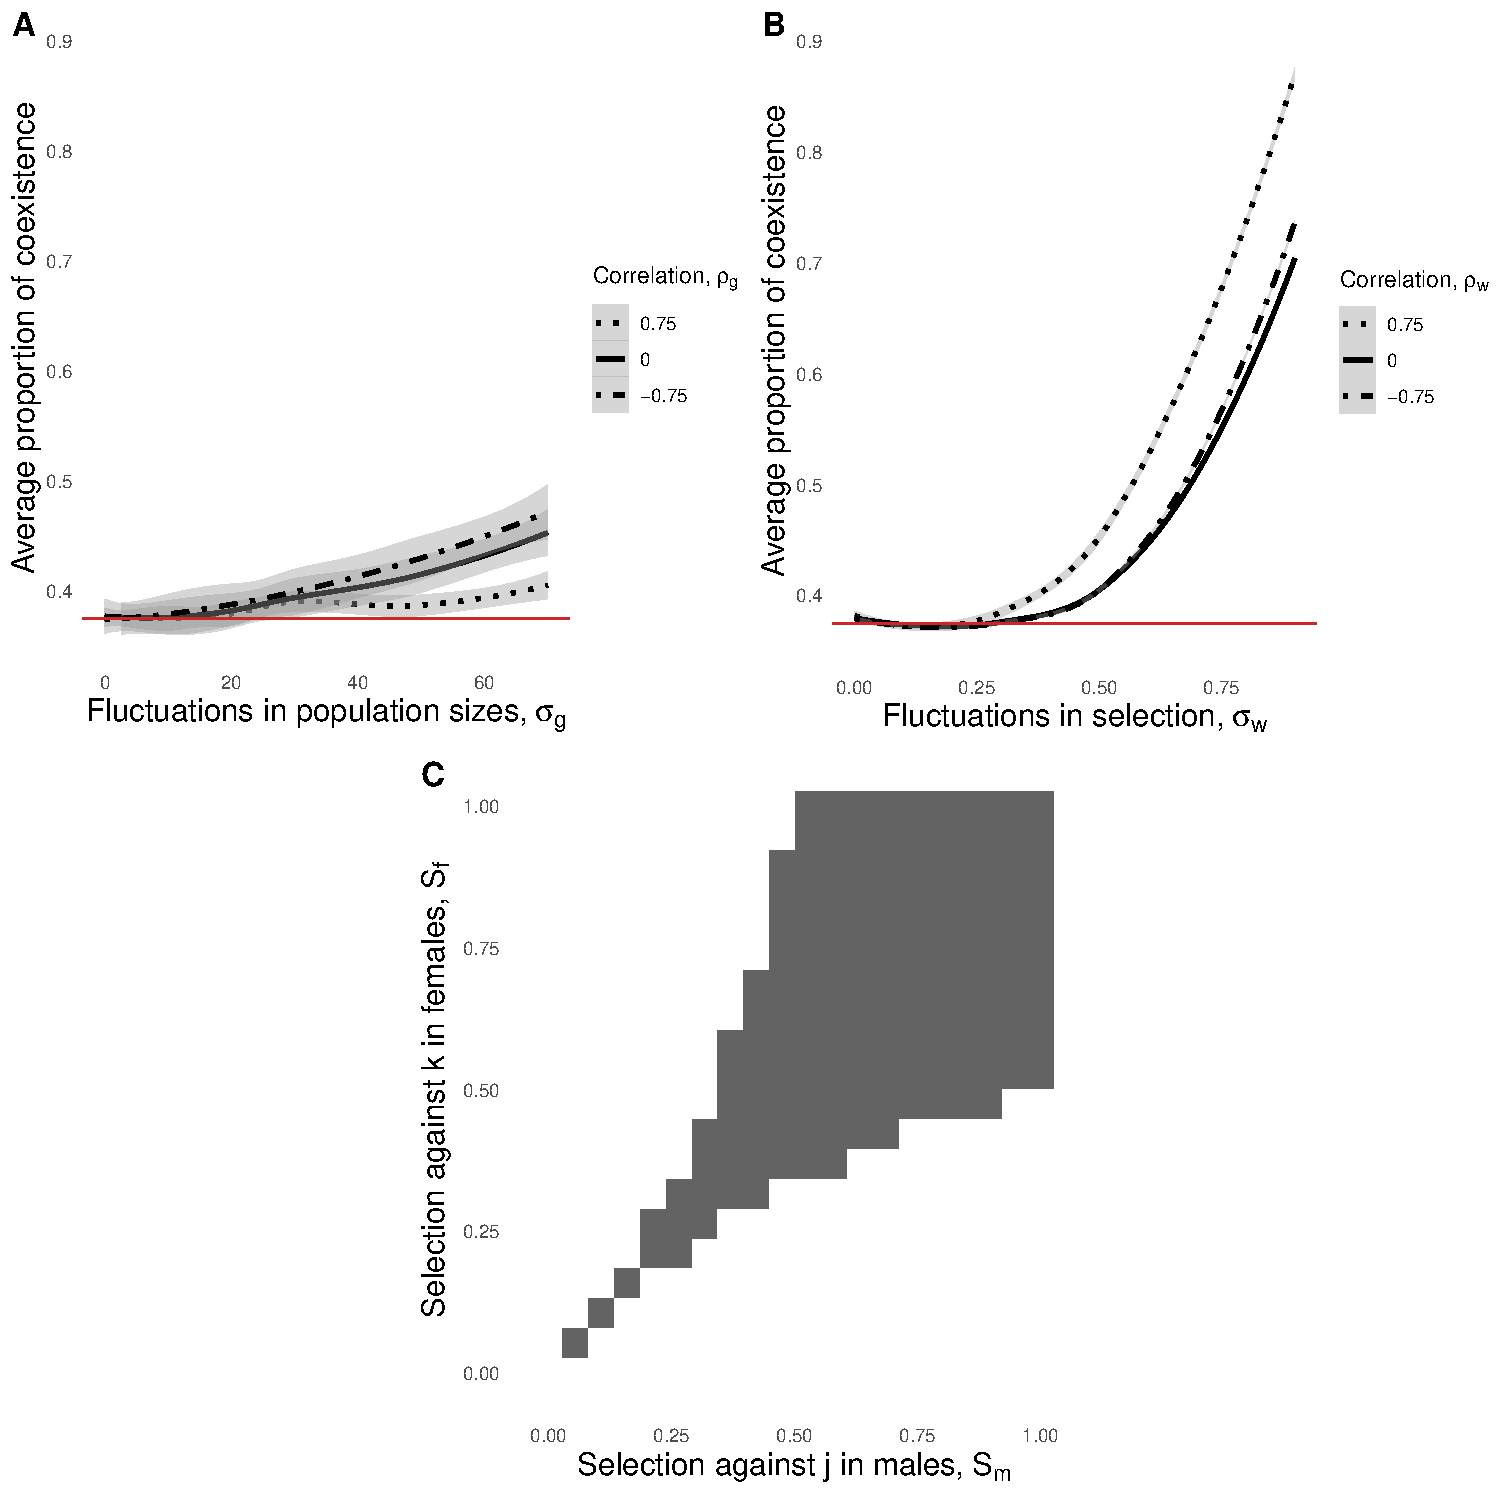
\includegraphics[width=1\textwidth]{proportions.pdf}}
%  \caption{ Changes in the proportion of coexistence as a function of fluctuations. In A) we show the results of  simulations in which only population sizes fluctuated (i.e., simulations in which $\sigma_{w}=0.001$ and $\rho_{w}= 0$). We show how the average proportion of coexistence, for all of the different invasion scenarios and replicates, changed as a function of the effect size of fluctuations in population sizes with black lines. We denoted the correlation between fluctuations in our simulations with different line types and displayed confident intervals around the average with shaded areas. The solid red line corresponds to the proportion of coexistence in the control simulation.  In B) we show the same results for simulations where only selection fluctuated  (i.e., simulations in which $\sigma_{g}=0.001$ and $\rho_{g}= 0$). Finally, in C) we show the results of the control simulation in the selection parameter space. Grey areas denote points in the parameter space where selection maintains both alleles in a population, which amount to $\approx 0.38$ of the selection parameter space, while white areas show competitive exclusion.}
%    \label{fig:prop}
%\end{figure}


\clearpage

\begin{figure}[H]
  \centerline{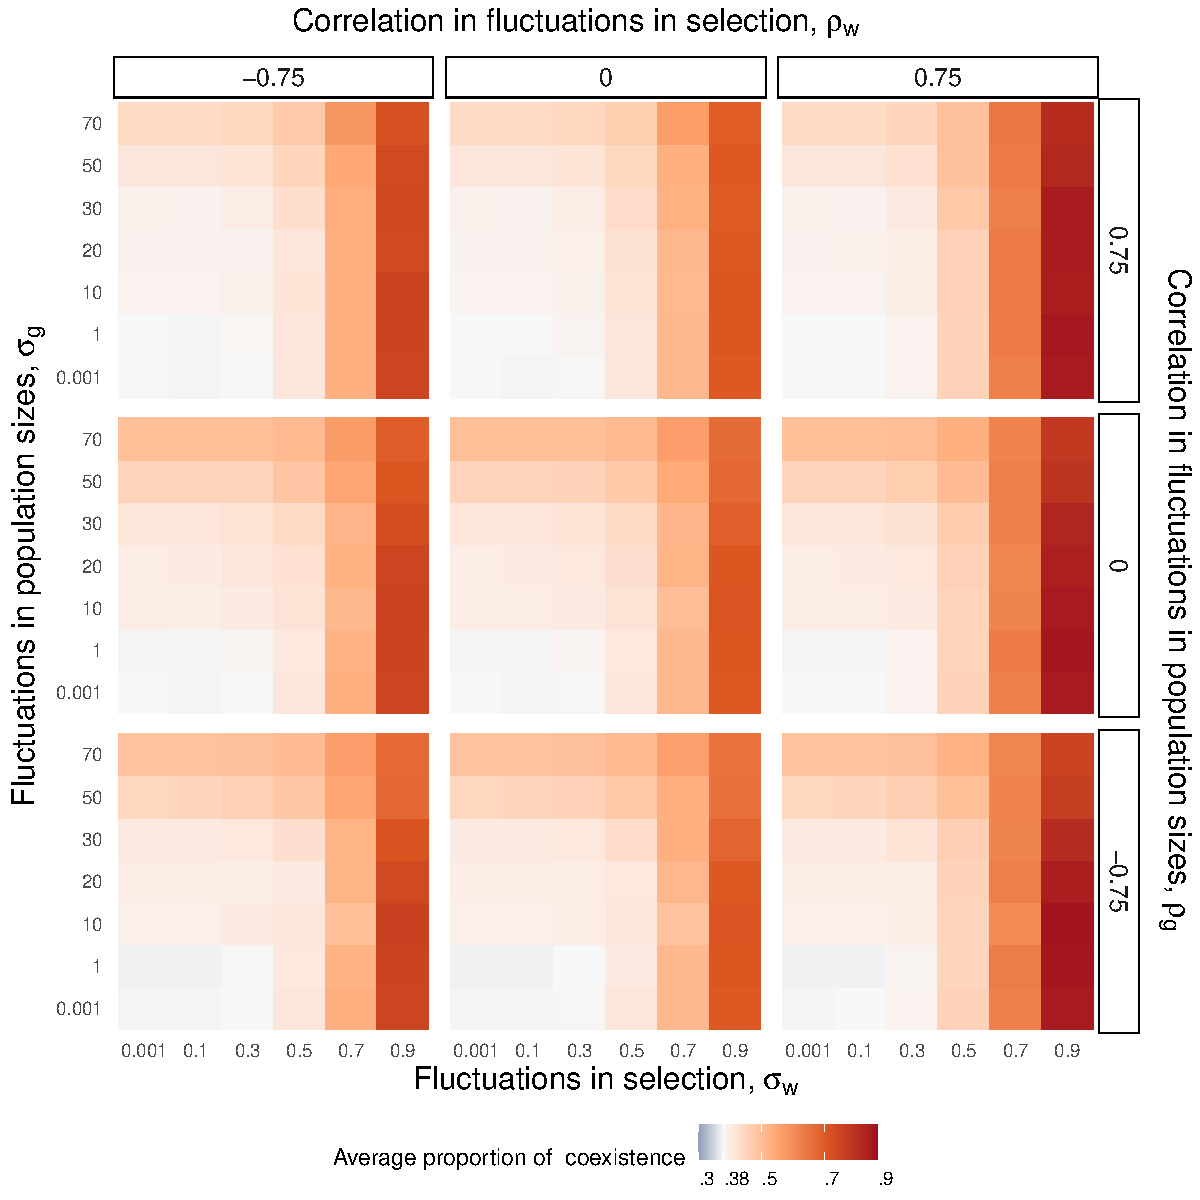
\includegraphics[width=1\textwidth]{heat_map.pdf}}
  \caption{The average proportion of coexistence across the selection parameter space. For all parameter combinations in our simulations, we show the average proportion of coexistence for all replicates and invasion scenarios (each allele invading a different sex). Each panel corresponds to a different combination of correlations between fluctuations. Labels on top indicate the correlation between fluctuations in selection $\rho_{w}$, while labels on the right show the correlation in fluctuations between fluctuations in population sizes $\rho_{g}$.  As a basis of comparison, we show the expected proportion of coexistence ($ 0.38$) as white in our color scheme.  }
    \label{fig:heatmap}
\end{figure}


\clearpage

\begin{figure}[H]
  \centerline{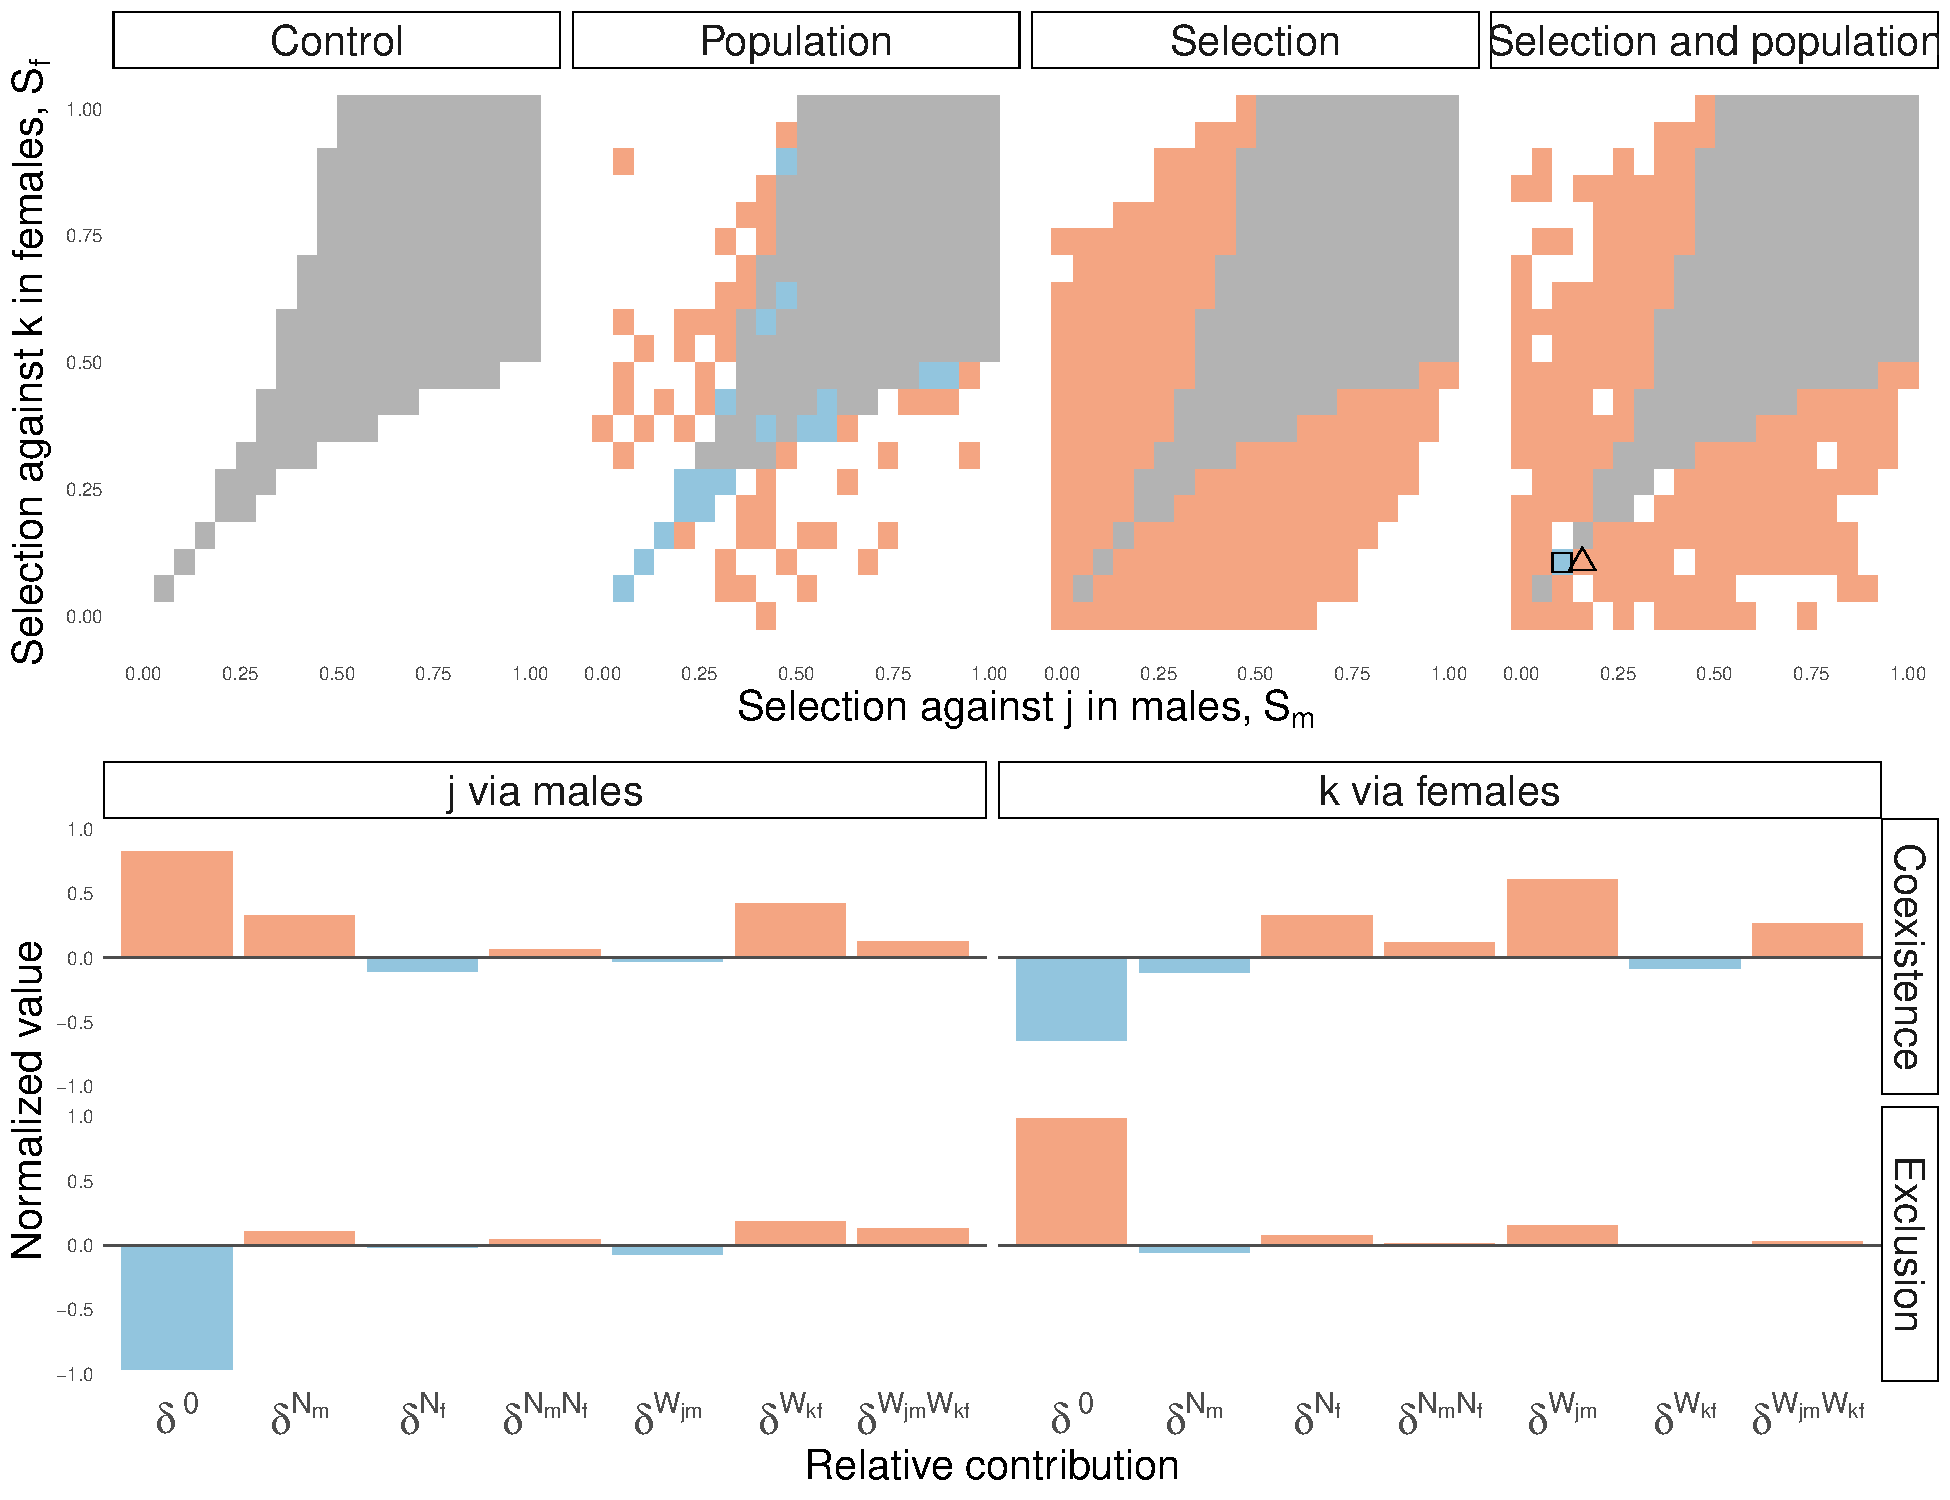
\includegraphics[width=1\textwidth]{outcomes.pdf}}
  \caption{  Coexistene outcomes and functional decomposition. In A) each panel corresponds to one replicate of a different type of simulation. All panels show the coexistence outcomes in the selection parameter space when $j$ invaded via males and $k$ invaded via females. As a reference, $j$ is favored in females and $k$ is favored in males. In the Control panel ($\sigma_{g}=0.001$, $\rho_{g}=0$, $\sigma_{w}=0.001$, $\rho_{w}=0$) grey areas indicate parts of the selection parameter space where alleles can coexist, while white areas indicate parts of the parameter space that correspond to competitive exclusion (following Eqn.\ref{selection}). In the Population ($\sigma_{g}=70$, $\rho_{g}=-0.75$, $\sigma_{w}=0.001$, $\rho_{w}=0$), Selection ($\sigma_{g}=0.001$, $\rho_{g}=0$, $\sigma_{w}=0.9$, $\rho_{w}=0.75$), and Selection and population ($\sigma_{g}=0.9$, $\rho_{g}=-0.75$, $\sigma_{w}=0.9$, $\rho_{w}=0.75$) panels, red areas indicate parts of the parameter space that ``flipped'' into coexistence, while  blue areas show changes into competitive exclusion. We highlighted two points in the parameter space in the Selection and popualtion panel that corresponded to changes into coexistence (triangle) and into competitive exlcusion (square).
   In B) we show the functional decomposition of the coexistence and competitive exclusion points highlighted in A). Each panel corresponds to each allele invading via their respective pathway and shows the bar plots of the different $\delta$ values that made up the functional decomposition of each allele as an invader. Red colors indicate positive $\delta$ values that benefited that allele as an invader more than the other allele as a resident, while  blue colors indicate negative $\delta$ values that benefited a resident more than the invader. }
    \label{fig:outcomes}
\end{figure}




\begin{figure}[H]
  \centerline{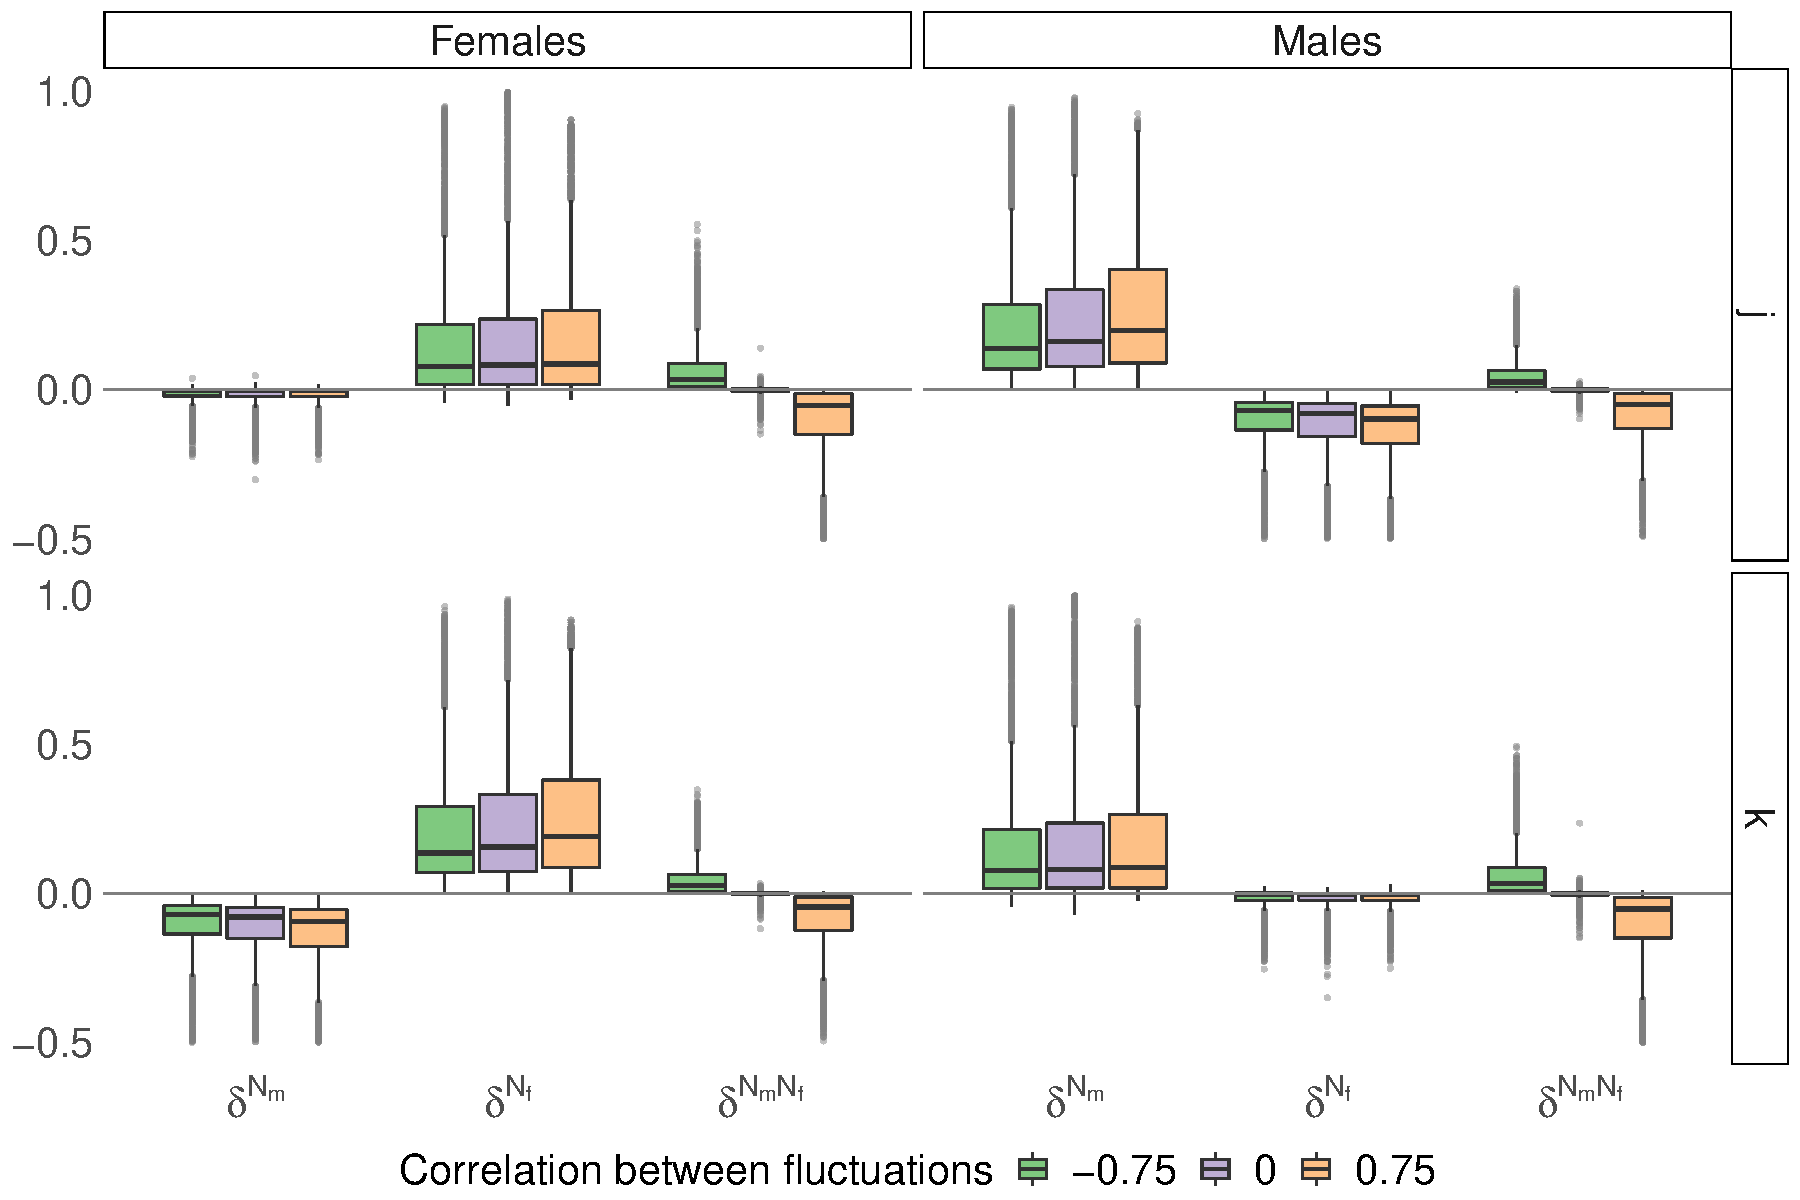
\includegraphics[width=1\textwidth]{box_plots.pdf}}
  \caption{The relative contributions of fluctuations in population sizes. Positive $\delta$ values imply that the corresponding fluctuation benefits that allele as an invader more than the other allele as a resident, negative $\delta$ values indicate fluctuations benefit the residents more than the invader, and $\delta$ values close to zero indicate that the corresponding fluctuation has equal contributions to invaders and residents. Each panel corresponds to each allele invading via a different pathway, for which we show the boxplots of the three distinct $\delta$ values that captured the effects of fluctuations in population sizes, for all of the replicates in our simulation in which $\sigma_{g}=70$. Each color corresponds to a different correlation between fluctuations in population sizes ($\rho_{g}$), as the legend indicates. Box plots extend from the first to third quantiles of the corresponding posterior distribution of parameter values, and the line inside the the box indicates the median. The upper whisker extends to the largest value no further than 1.5 times the inter-quantile range (IQR, or the distance between the first and third quartiles); the lower whisker extends to the smallest value at most 1.5 times the IQR. Data beyond the end of the whiskers are determined to be outliers and are plotted individually with solid grey points. }
    \label{fig:boxes}
\end{figure}



\begin{figure}[H]
  \centerline{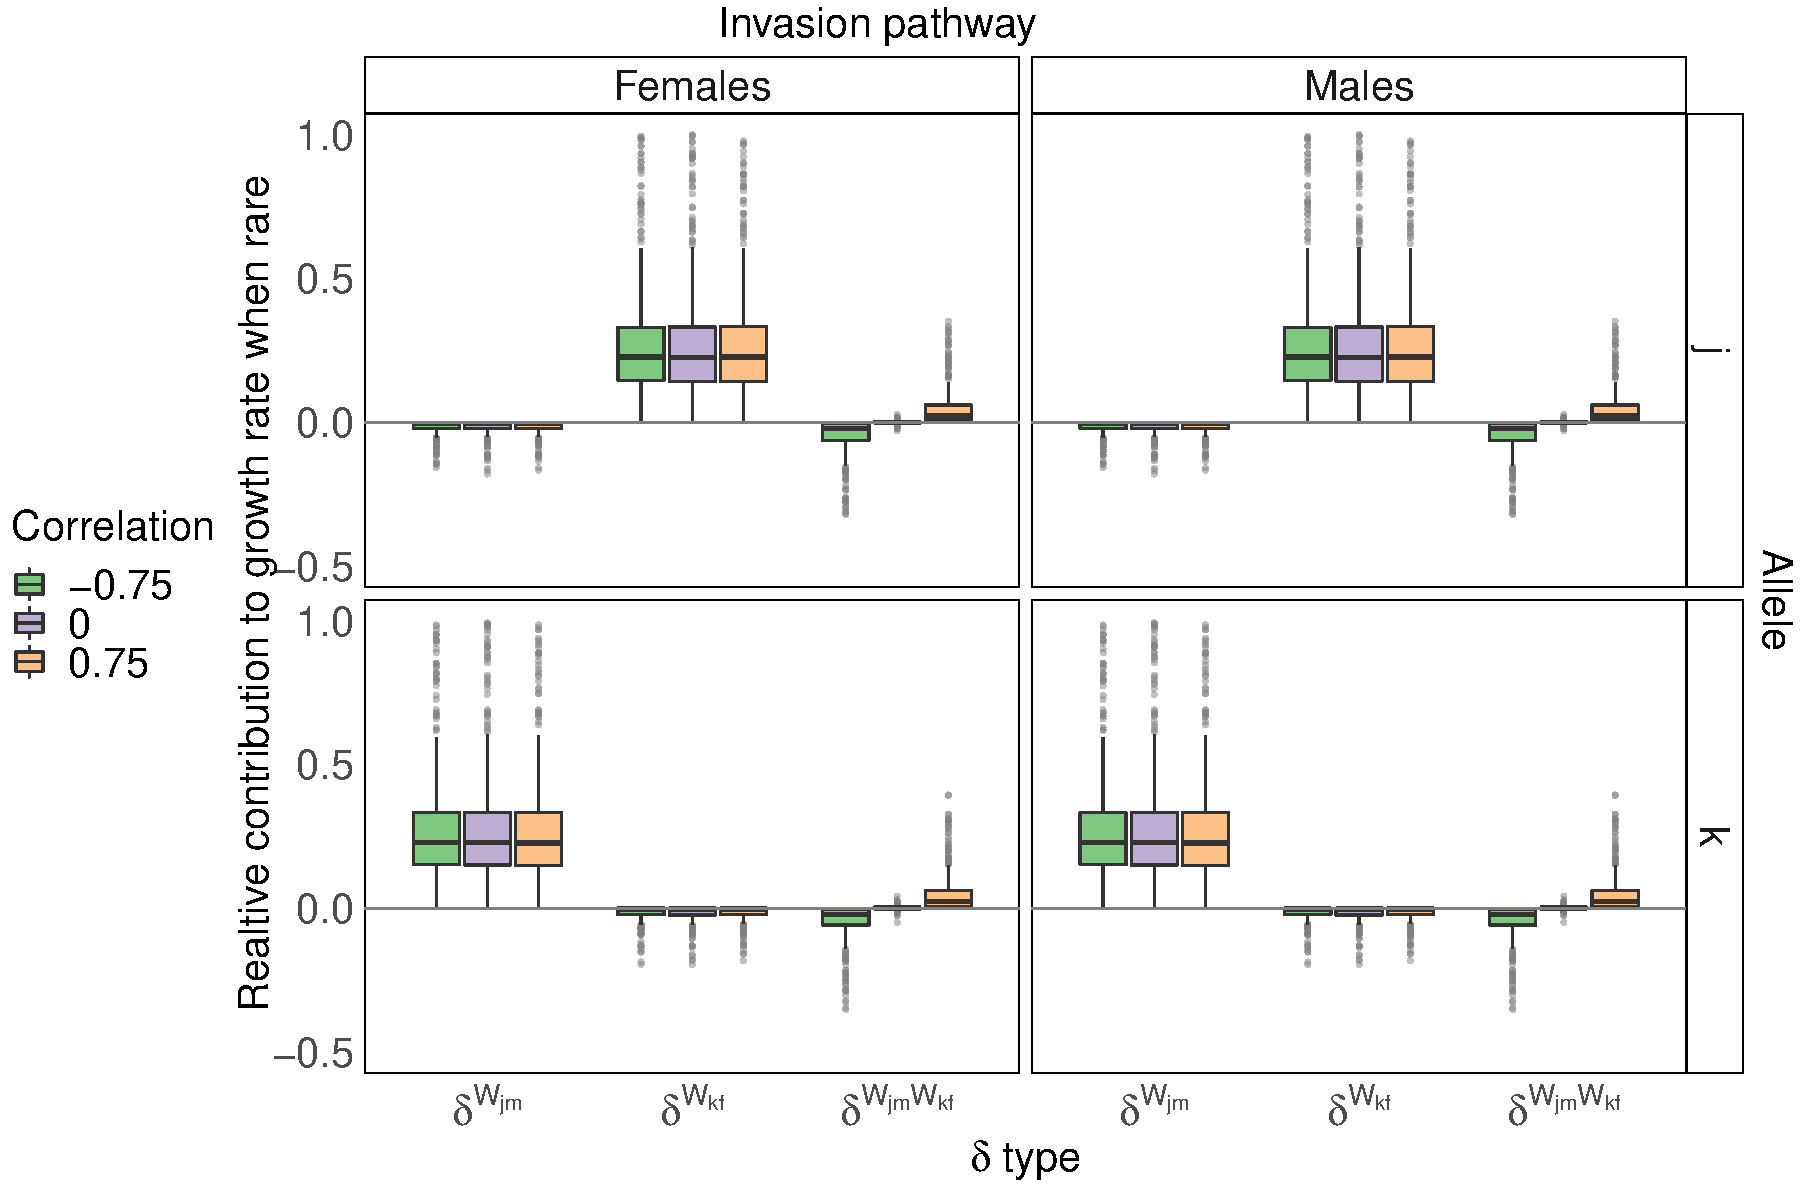
\includegraphics[width=1\textwidth]{box_plots_selection.pdf}}
  \caption{ The relative contributions of fluctuations in selection. As a reference, positive $\delta$ values imply that the corresponding fluctuation benefits that allele as an invader more than the other allele as a resident, negative $\delta$ values indicate fluctuations benefit the residents more than the invader, and $\delta$ values close to zero indicate that the corresponding fluctuation has equal contributions to invaders and residents. Each panel corresponds to each allele invading via a different pathway, for which we show the boxplots of the three distinct $\delta$ values that captured the effects of fluctuations in population sizes, for all of the replicates in our simulation in which $\sigma_{w}=0.90$. Each color corresponds to a different correlation between fluctuations in population sizes ($\rho_{w}$), as the legend indicates. Box plots extend from the first to third quantiles of the corresponding posterior distribution of parameter values, and the line inside the the box indicates the median. The upper whisker extends to the largest value no further than 1.5 times the inter-quantile range (IQR, or the distance between the first and third quartiles); the lower whisker extends to the smallest value at most 1.5 times the IQR. Data beyond the end of the whiskers are determined to be outliers and are plotted individually with solid grey points.  }
    \label{fig:boxes_selection}
\end{figure}
